\documentclass[a4paper,14pt]{extarticle}

\usepackage[a4paper,top=20mm,bottom=20mm,left=30mm,right=10mm]{geometry}
\usepackage[T1,T2A]{fontenc}
\usepackage[utf8]{inputenc}
\usepackage[russian]{babel}
\usepackage{indentfirst}
\usepackage{titlesec}
\usepackage{graphicx}
\usepackage{verbatim}
\usepackage{fancyvrb}

\renewcommand{\baselinestretch}{1.3}
\titleformat{\section}{\normalsize\bfseries}{\thesection}{1em}{}
\titleformat{\subsection}{\normalsize\bfseries}{\thesection}{1em}{}
\setlength{\parindent}{12.5mm}

\begin{document}

	\newpage\thispagestyle{empty}
	\begin{center}
		\MakeUppercase{
			Министерство науки и высшего образования Российской Федерации\\
			Федеральное государственное бюджетное образовательное учреждение высшего образования\\
			<<Вятский Государственный Университет>>\\
		}
		Институт математики и информационных систем\\
		Факультет автоматики и вычислительной техники\\
		Кафедра электронных вычислительных машин
	\end{center}
	\vfill
	
	\begin{center}
		Отчет по лабораторной работе №5\\
		по дисциплине\\
		<<Программирование>>\\
	\end{center}
	\vfill
	
	\noindent
	\begin{tabular}{ll}
		Выполнил студент гр. ИВТб-1301-05-00 \hspace{5mm} &
		\rule[-1mm]{25mm}{0.10mm}\,/Макаров С.А./\\
		
		Руководитель зав. кафедры ЭВМ & \rule[-1mm]{25mm}{0.10mm}\,/Долженкова М.Л./\\
	\end{tabular}
	
	\vfill
	\begin{center}
		Киров 2025
	\end{center}
	
	\newpage
	\section*{Цель}
	Цель лабораторной работы: получить базовые сведения о наиболее известных алгоритмах сортировки, изучить принципы работы с текстовыми файлами.
	
	\section*{Задание}
	\begin{enumerate}
		\item Реализовать сортировку данных с помощью алгоритма подсчётом.
		
		\item Реализовать сортировку данных с помощью поразрядного алгоритма.
		
		\item В обоих случаях необходимо предусмотреть возможность изменения компаратора (реализация компаратора в виде передаваемой в подпрограмму функции).
		
		\item Считывание и вывод данных необходимо производить из текстового файла.
		
		\item Для демонстрации работы программных реализаций самостоятельно подготовить варианты входных данных (при этом объем тестовых файлов должен позволять оценить скорость работы программ).
	\end{enumerate}
	
	\pagebreak
	\section*{Решение}

	\begin{figure}[h]
		\centering
		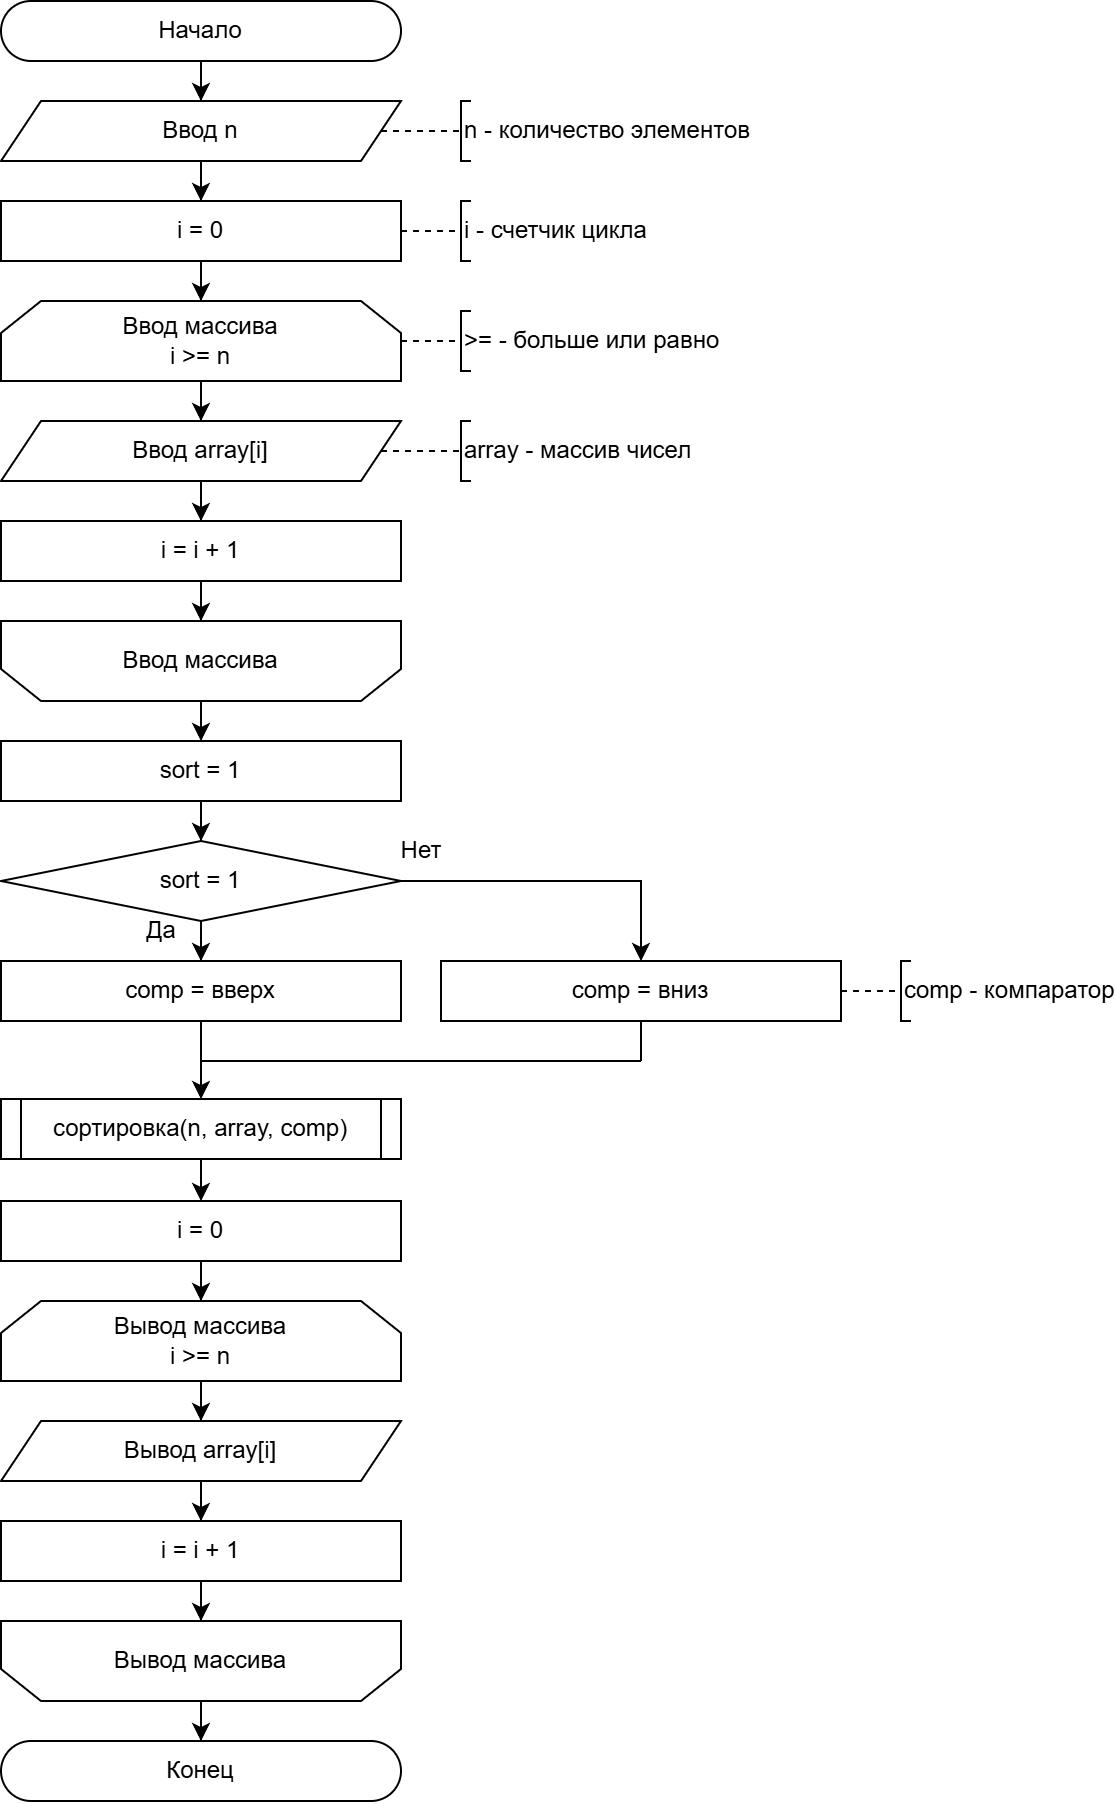
\includegraphics[width=0.7\linewidth]{images/s-1-1}
	\end{figure}
	\begin{center}
		Рисунок 1 – Схема алгоритма сортировки подсчетом
	\end{center}

	\pagebreak
	\begin{figure}[h]
		\centering
		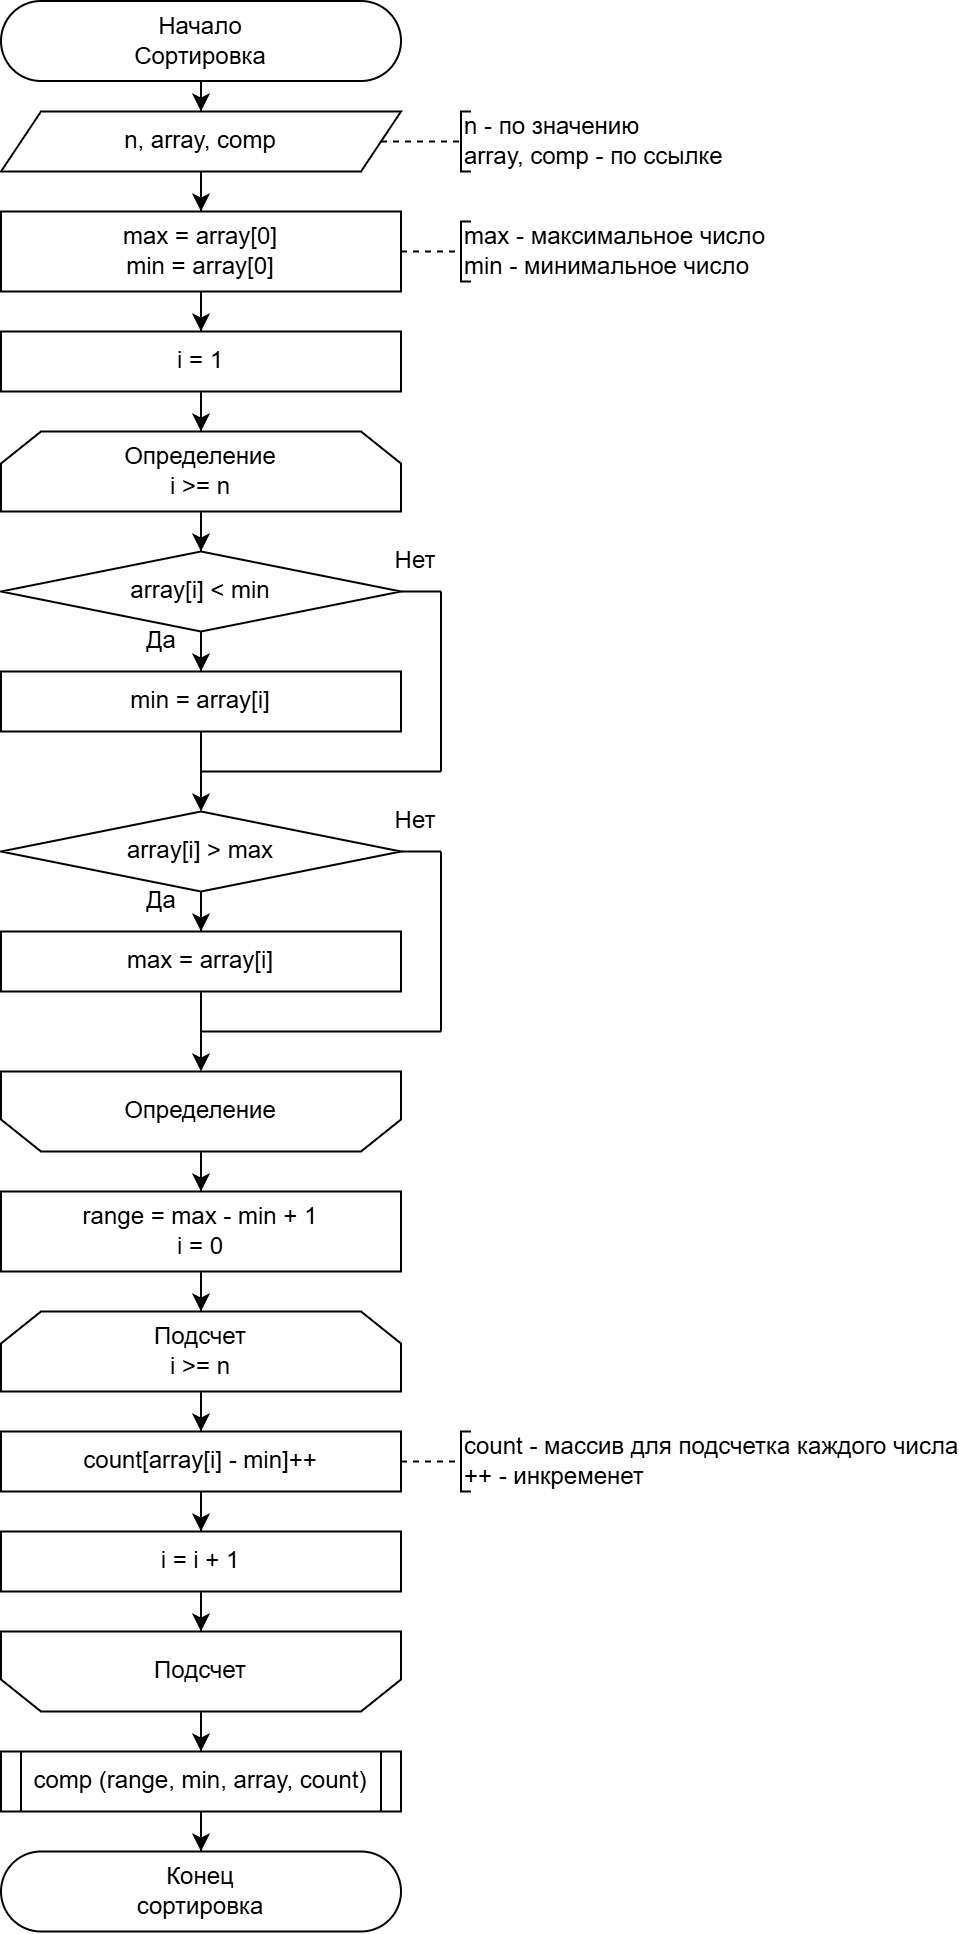
\includegraphics[width=0.58\linewidth]{images/s-1-2}
	\end{figure}
	\begin{center}
		Рисунок 2 – Схема алгоритма подпрограммы <<Сортировка>>
	\end{center}

	\pagebreak
	\begin{figure}[h]
		\centering
		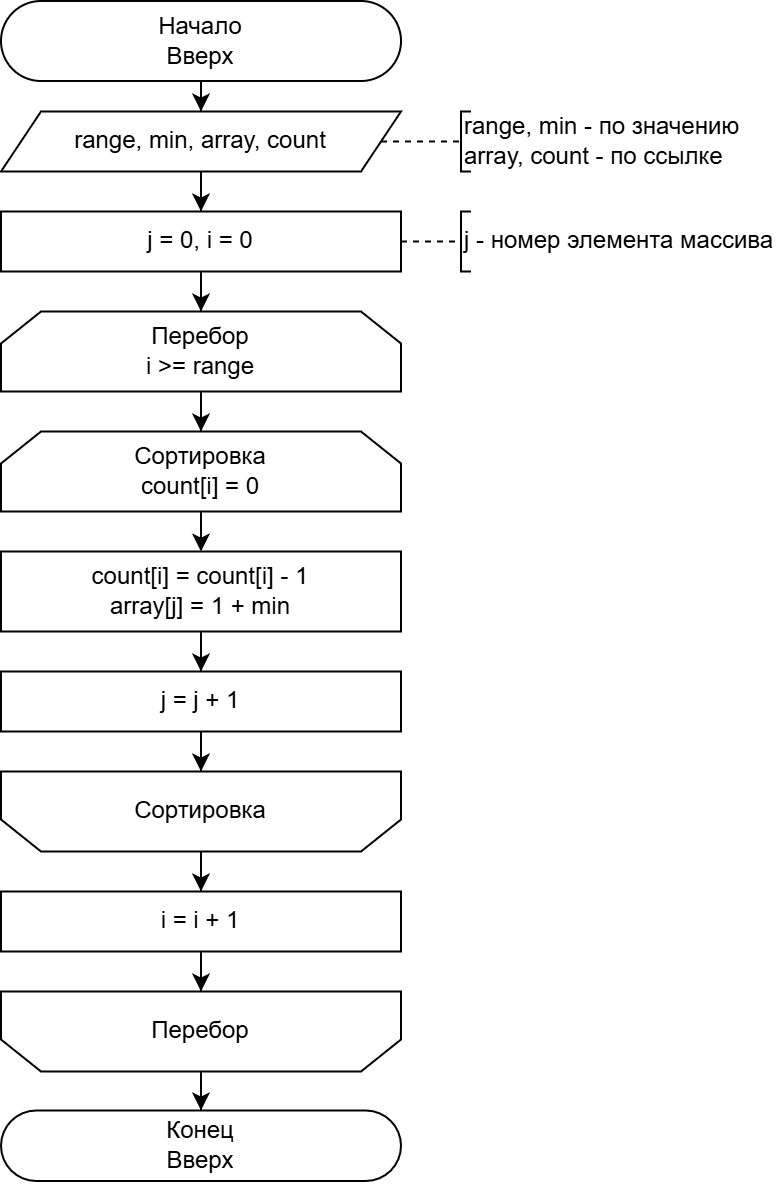
\includegraphics[width=0.6\linewidth]{images/s-1-3}
	\end{figure}
	\begin{center}
		Рисунок 3 – Схема алгоритма подпрограммы <<Вверх>>
	\end{center}

	\pagebreak
	\begin{figure}[h]
		\centering
		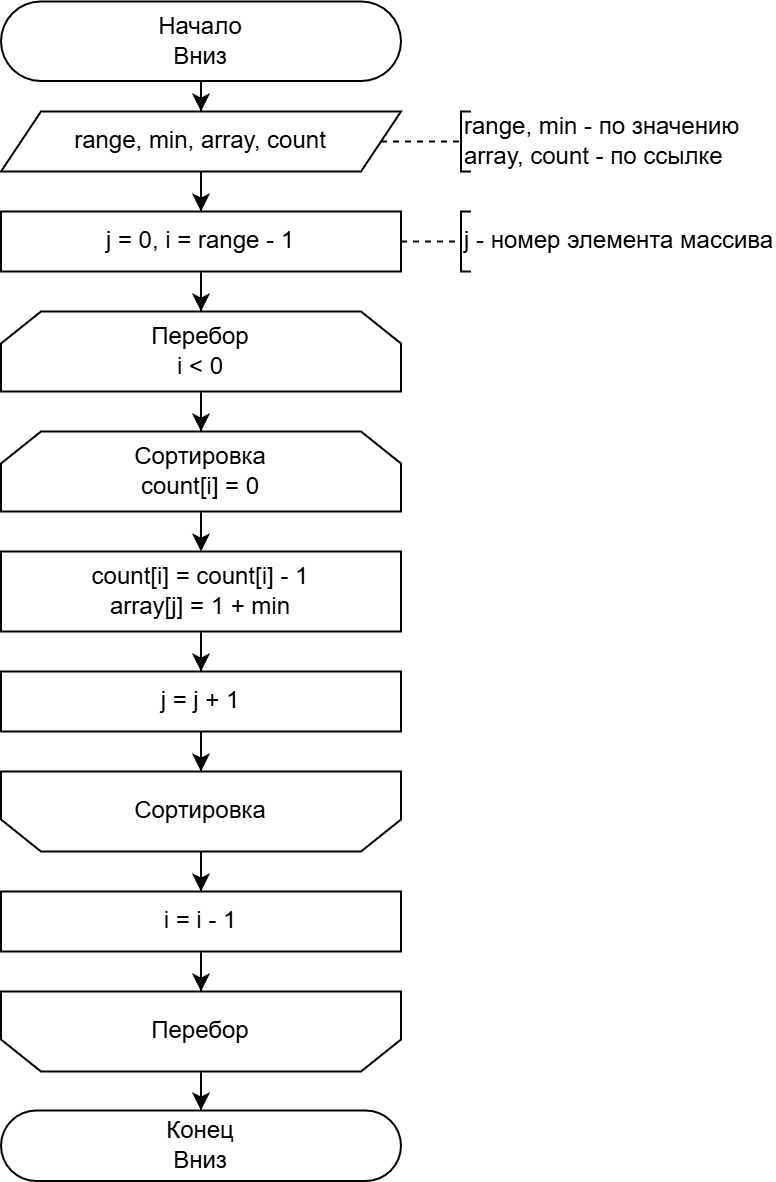
\includegraphics[width=0.6\linewidth]{images/s-1-4}
	\end{figure}
	\begin{center}
		Рисунок 4 – Схема алгоритма подпрограммы <<Вниз>>
	\end{center}

	\noindent
	\begin{Verbatim}[tabsize=4,fontsize=\small]
#include <stdio.h>
#include <stdlib.h>
void sort(int n, int array[], 
	void(*comparator)(int range, int min, int array[], int count[])) {
	int min = array[0];
	int max = array[0];
	for (int i = 1; i < n; i++) {
		if (array[i] < min) min = array[i];
		if (array[i] > max) max = array[i];
	}
	int range = max - min + 1;
	int* count = (int*)calloc(range, sizeof(int));
	for (int i = 0; i < n; i++) count[array[i] - min]++;
	comparator(range, min, array, count);
}
void comparatorUp(int range, int min, int array[], int count[]) {
	int j = 0;
	for (int i = 0; i < range; i++) {
		while (count[i] > 0) {
			count[i]--;
			array[j++] = i + min;
		}
	}
}
void comparatorDown(int range, int min, int array[], int count[]) {
	int j = 0;
	for (int i = range - 1; i >= 0; i--) {
		while (count[i] > 0) {
			count[i]--;
			array[j++] = i + min;
		}
	}
}
int main() {
	FILE* input = fopen("../input.txt", "r");
	FILE* output = fopen("../output.txt", "w");
	int n = 0;
	fscanf_s(input, "%d", &n);
	int* array = (int*)calloc(n, sizeof(int));
	for (int i = 0; i < n; i++) fscanf_s(input, "%d", &array[i]);
	fclose(input);
	void(*comparator)(int range, int min, int array[], int count[]);
	comparator = comparatorUp;
	sort(n, array, comparator);
	for (int i = 0; i < n; i++) {
		fprintf(output, "%d ", array[i]);
	}
	fclose(output);
	free(array);
	return 0;
}
	\end{Verbatim}

	\pagebreak
	\begin{figure}[h]
		\centering
		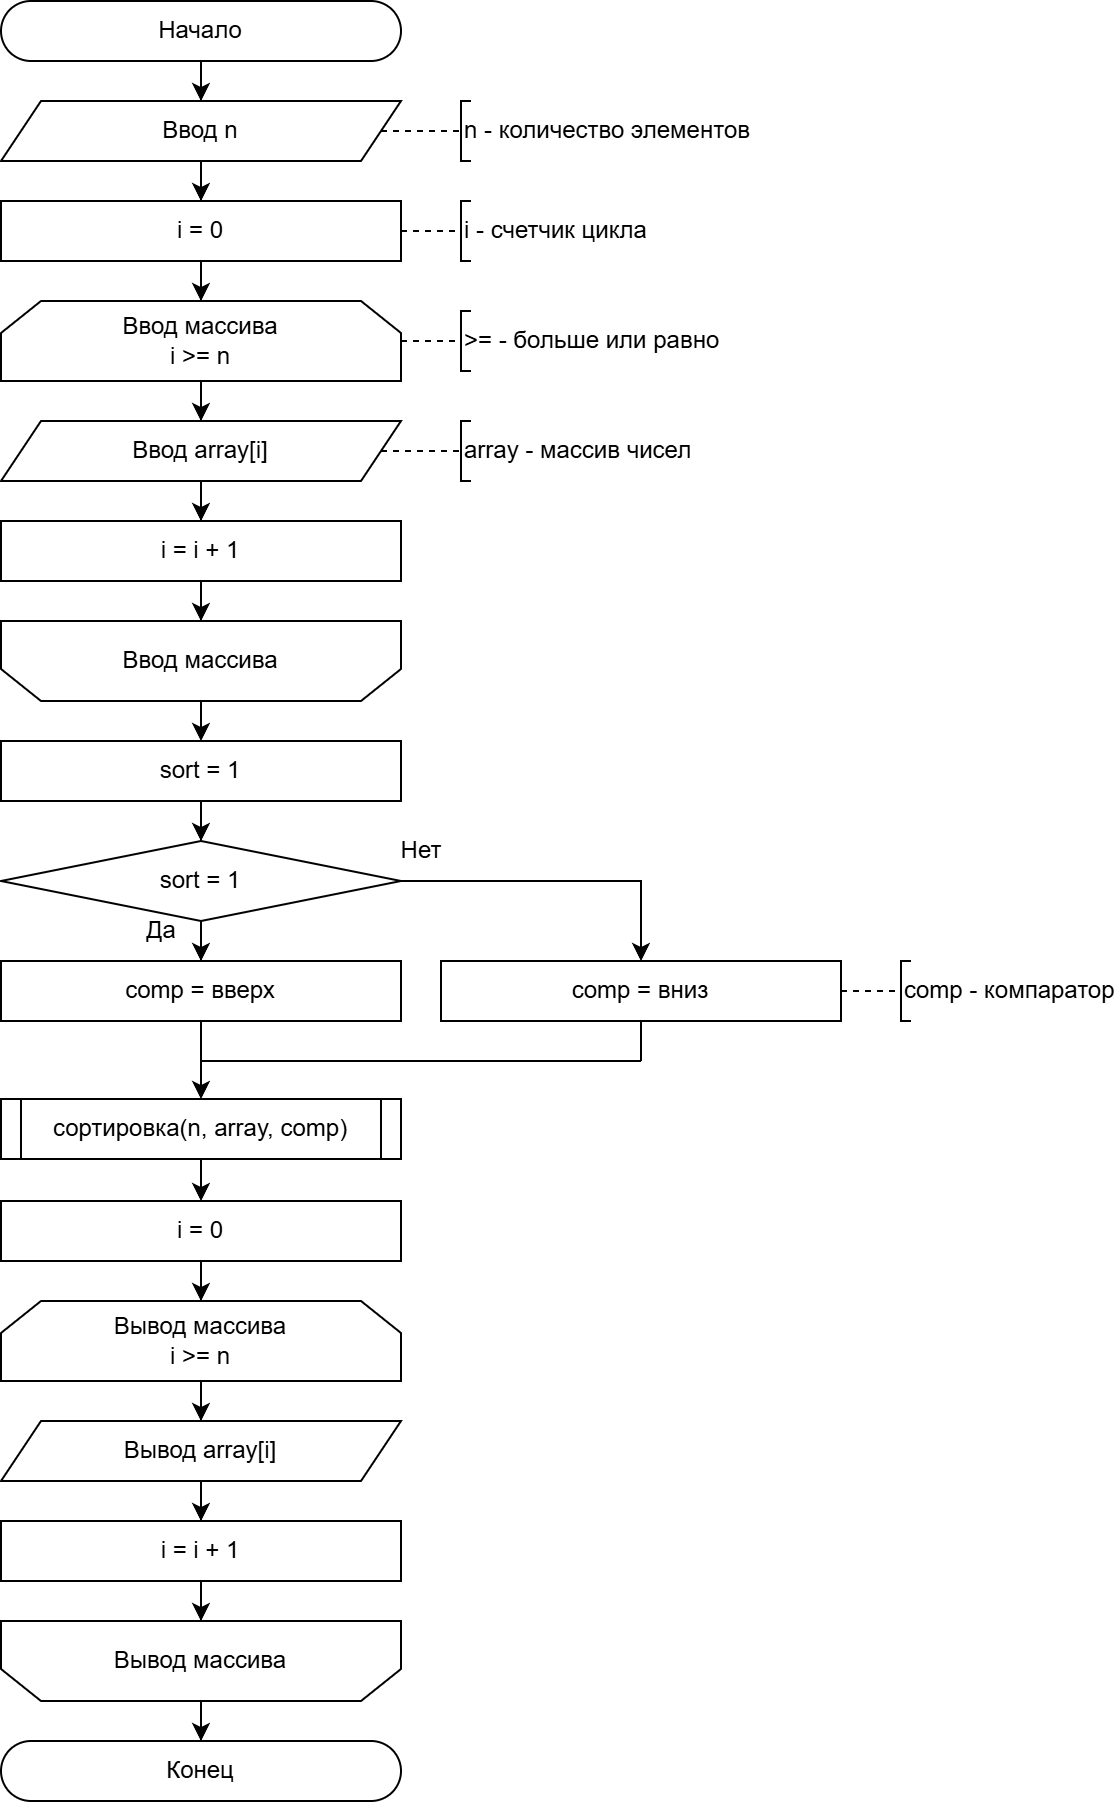
\includegraphics[width=0.7\linewidth]{images/s-2-1}
	\end{figure}
	\begin{center}
		Рисунок 5 – Схема алгоритма поразрядной сортировки
	\end{center}

	\pagebreak
	\begin{figure}[h]
		\centering
		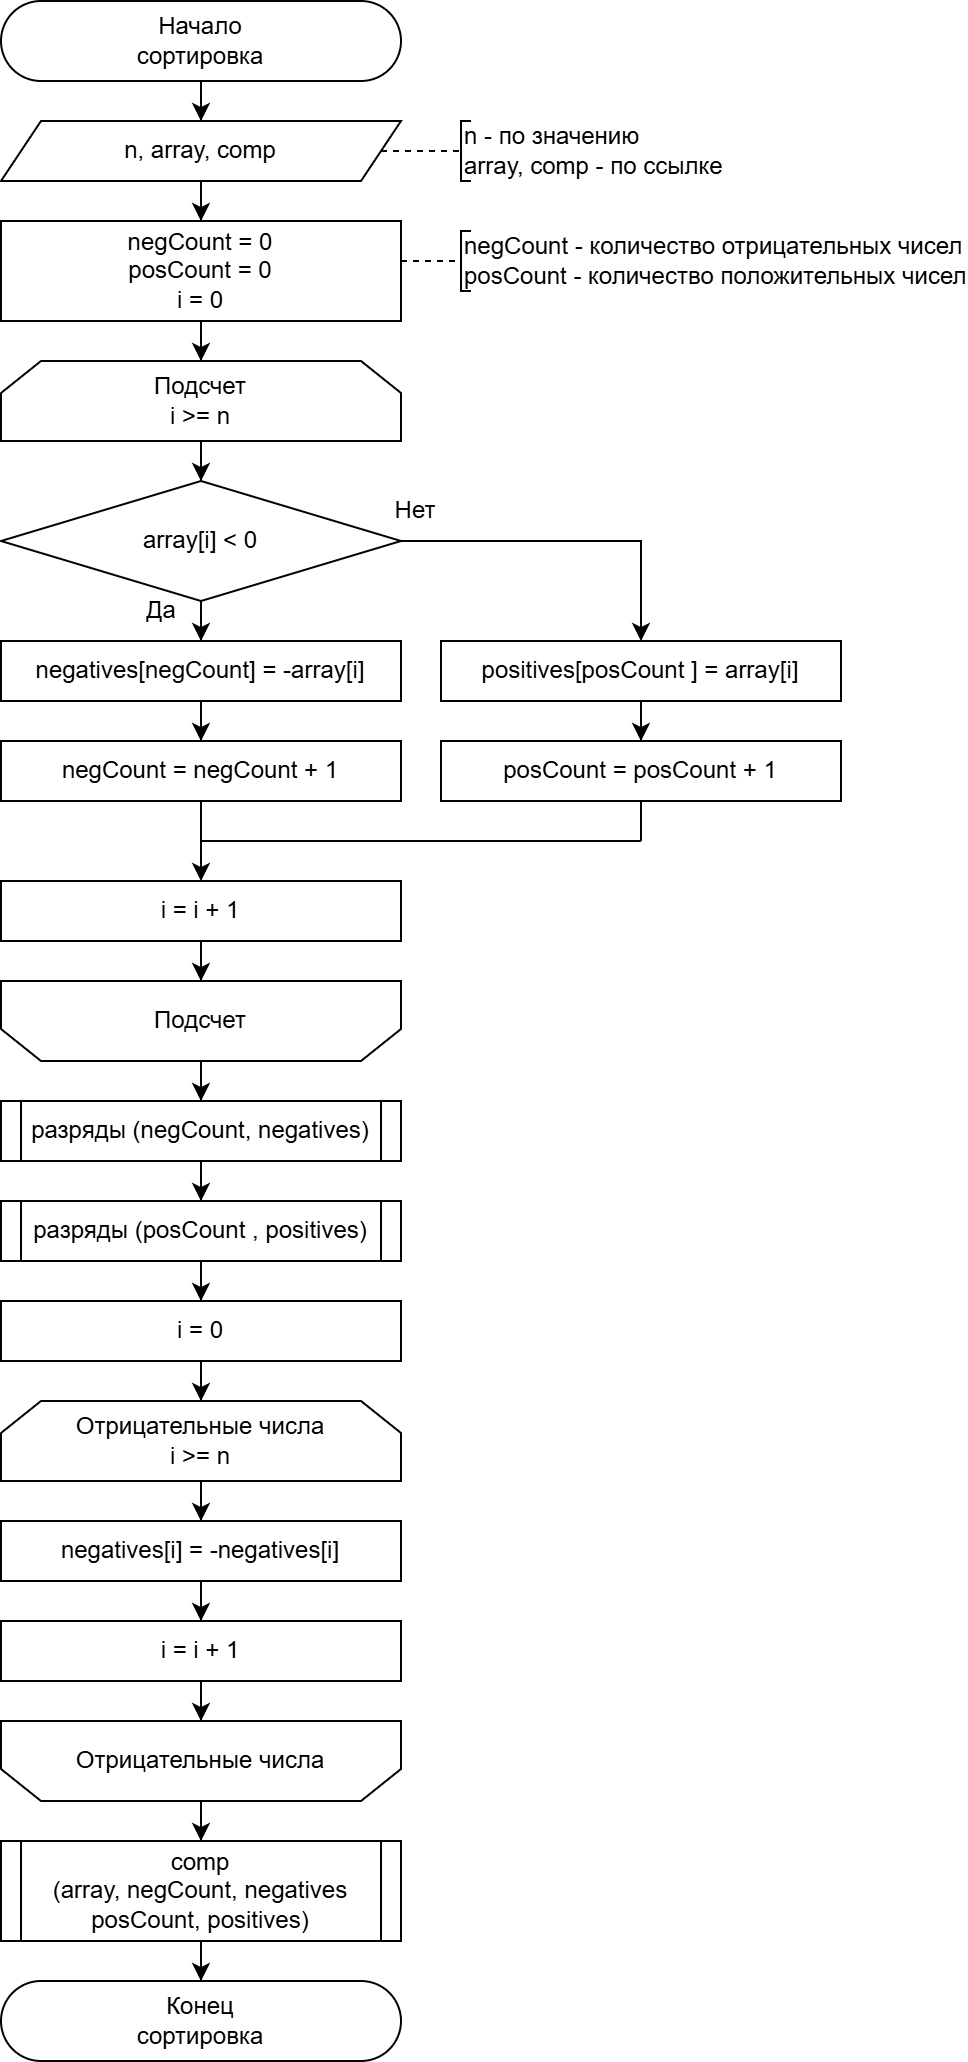
\includegraphics[width=0.55\linewidth]{images/s-2-2}
	\end{figure}
	\begin{center}
		Рисунок 6 – Схема алгоритма подпрограммы <<Сортировка>>
	\end{center}

	\pagebreak
	\begin{figure}[h]
		\centering
		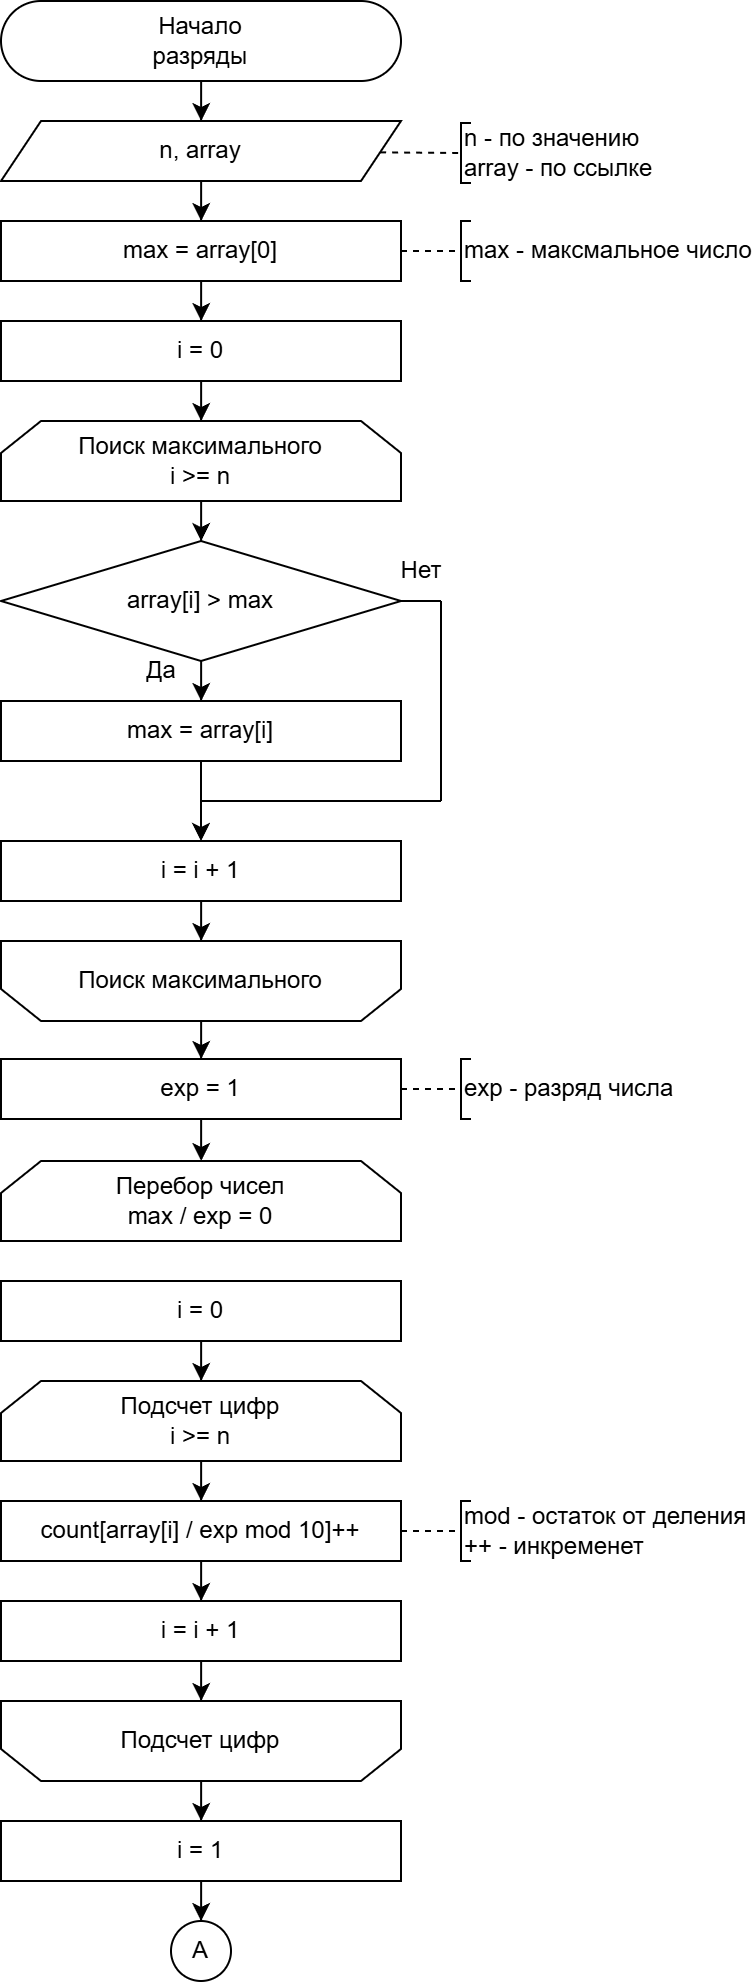
\includegraphics[width=0.43\linewidth]{images/s-2-3}
	\end{figure}
	\begin{center}
		Рисунок 7 – Схема алгоритма подпрограммы <<Разряды>>
	\end{center}

	\pagebreak
	\begin{figure}[h]
		\centering
		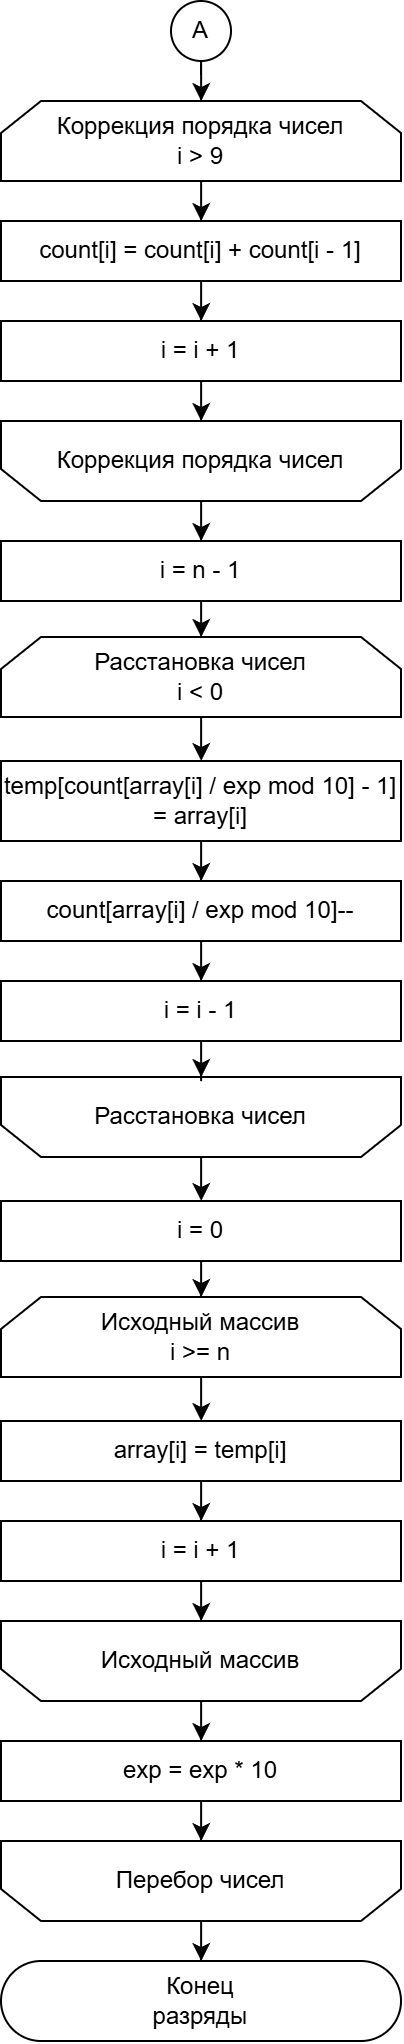
\includegraphics[width=0.23\linewidth]{images/s-2-4}
	\end{figure}
	\begin{center}
		Рисунок 8 – Продолжение схемы алгоритма подпрограммы <<Разряды>>
	\end{center}

	\pagebreak
	\begin{figure}[h]
		\centering
		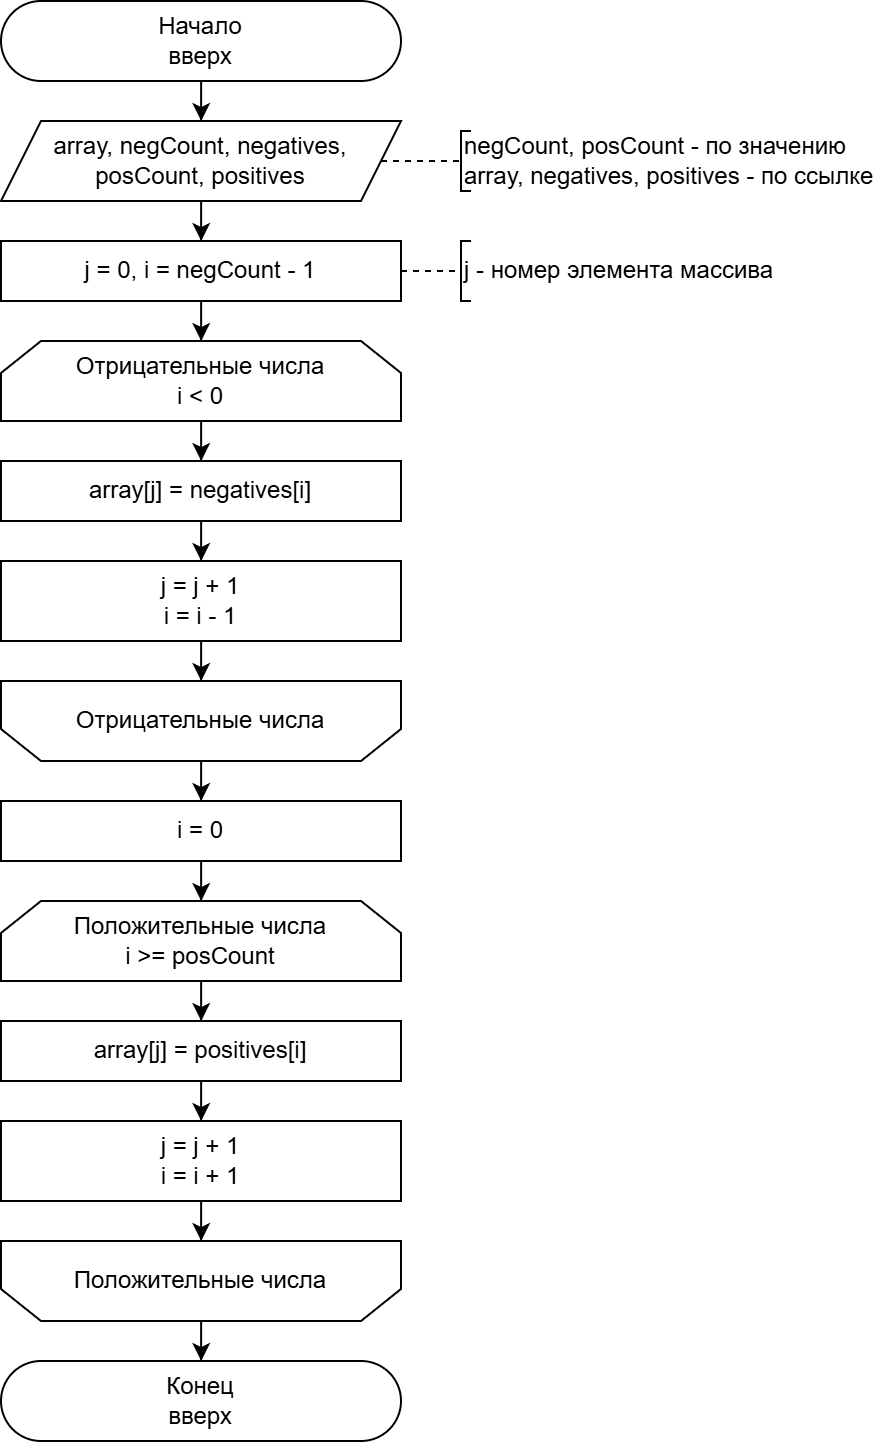
\includegraphics[width=0.65\linewidth]{images/s-2-5}
	\end{figure}
	\begin{center}
		Рисунок 9 – Схема алгоритма подпрограммы <<Вверх>>
	\end{center}

	\pagebreak
	\begin{figure}[h]
		\centering
		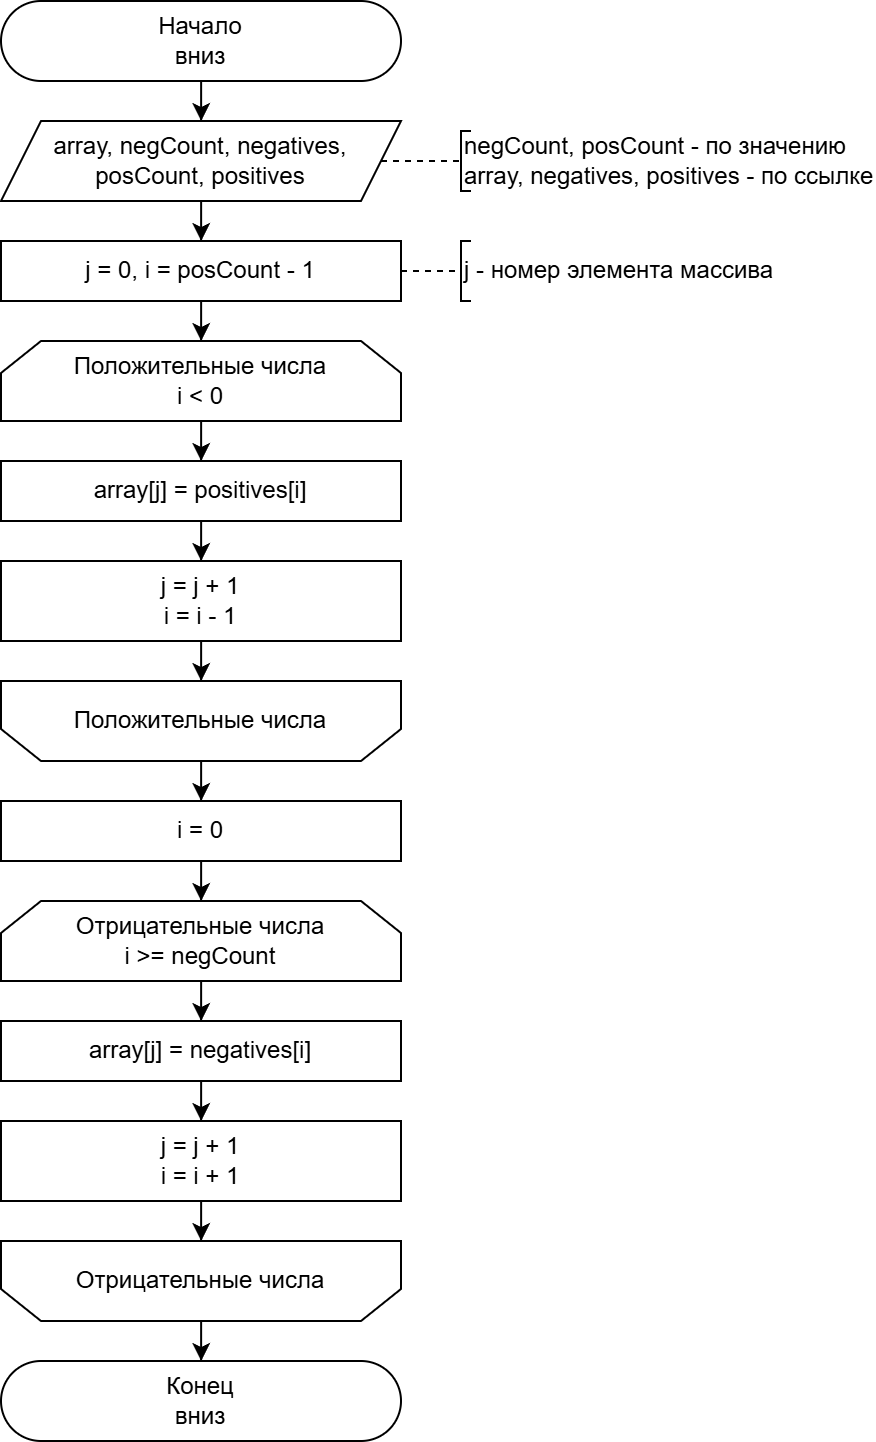
\includegraphics[width=0.65\linewidth]{images/s-2-6}
	\end{figure}
	\begin{center}
		Рисунок 10 – Схема алгоритма подпрограммы <<Вниз>>
	\end{center}

	\noindent
	\begin{Verbatim}[tabsize=4,fontsize=\small]
#include <stdio.h>
#include <stdlib.h>
void radixSort(int n, int array[]) {
	int max = array[0];
	for (int i = 1; i < n; i++) {
		if (array[i] > max) max = array[i];
	}
	for (int exp = 1; max / exp > 0; exp *= 10) {
		int* temp = (int*)calloc(n, sizeof(int));
		int count[10] = { 0 };
		for (int i = 0; i < n; i++) {
			count[array[i] / exp % 10]++;
		}
		for (int i = 1; i < 10; i++) {
			count[i] += count[i - 1];
		}
		for (int i = n - 1; i >= 0; i--) {
			temp[count[array[i] / exp % 10] - 1] = array[i];
			count[array[i] / exp % 10]--;
		}
		for (int i = 0; i < n; i++) {
			array[i] = temp[i];
		}
	}
}
void sort(int n, int array[], 
	void(*comparator)(int array[], 
		int negCount, int negatives[], int posCount, int positives[])) {
	int* negatives = (int*)calloc(n, sizeof(int));
	int* positives = (int*)calloc(n, sizeof(int));
	int negCount = 0, posCount = 0;
	for (int i = 0; i < n; i++) {
		if (array[i] < 0) {
			negatives[negCount++] = -array[i];
		} else {
			positives[posCount++] = array[i];
		}
	}
	radixSort(negCount, negatives);
	radixSort(posCount, positives);
	for (int i = 0; i < negCount; i++) {
		negatives[i] = -negatives[i];
	}
	comparator(array, negatives, negCount, positives, posCount);
	free(negatives);
	free(positives);
}
void comparatorUp(int array[], int negCount, int negatives[], 
	int posCount, int positives[]) {
	int j = 0;
	for (int i = negCount - 1; i >= 0; i--) {
		array[j++] = negatives[i];
	}
	for (int i = 0; i < posCount; i++) {
		array[j++] = positives[i];
	}
}
void comparatorDown(int array[], int negCount, int negatives[],
	int posCount, int positives[]) {
	int j = 0;
	for (int i = posCount - 1; i >= 0; i--) {
		array[j++] = positives[i];
	}
	for (int i = 0; i < negCount; i++) {
		array[j++] = negatives[i];
	}
}
int main() {
	FILE* input = fopen("../input.txt", "r");
	FILE* output = fopen("../output.txt", "w");
	int n = 0;
	fscanf_s(input, "%d", &n);
	int* array = (int*)calloc(n, sizeof(int));
	for (int i = 0; i < n; i++) fscanf_s(input, "%d", &array[i]);
	fclose(input);
	void(*comparator)(int array[], int negCount, 
		int negatives[], int posCount, int positives[]);
	comparator = comparatorUp;
	sort(n, array, comparator);
	for (int i = 0; i < n; i++) {
		fprintf(output, "%d ", array[i]);
	}
	fclose(output);
	free(array);
	return 0;
}
	\end{Verbatim}
	
	\section*{Вывод}
	В ходе выполнения лабораторной работы были изучены алгоритмы сортировки подсчётом и поразрядной сортировки по младшим разрядам. Также были изучены принципы работы с текстовыми файлами путём решения предложенных задач.

\end{document}